%
% 6.006 problem set 6 solutions template
%
\documentclass[12pt,twoside]{article}

\newcommand{\name}{}

\usepackage{amssymb}
\usepackage{amsmath}
\usepackage{graphicx}
\usepackage{latexsym}
\usepackage{times,url}
\usepackage{cprotect}
\usepackage{listings}
\usepackage{graphicx}
\usepackage[table]{xcolor}
\usepackage[letterpaper]{geometry}
\usepackage{tikz-qtree}
\usepackage{enumerate}

\newcommand{\profs}{Instructors: Erik Demaine, Jason Ku, and Justin Solomon}
\newcommand{\subj}{6.006}
\newcommand{\ttt}[1]{{\tt\small #1}}

\definecolor{dkgreen}{rgb}{0,0.6,0}
\definecolor{dkblue}{rgb}{.2,.2,1}
\definecolor{gray}{rgb}{0.5,0.5,0.5}
\definecolor{mauve}{rgb}{0.58,0,0.82}

\lstset{
  language=Python,
  aboveskip=1pc,
  belowskip=1pc,
  basicstyle={\footnotesize\ttfamily},
  numbers=left,
  showstringspaces=false,
  numberstyle={\tiny\color{gray}\ttfamily},
  keywordstyle={\color{dkblue}\ttfamily},
  commentstyle={\color{dkgreen}\ttfamily},
  stringstyle={\color{mauve}\ttfamily},
}

% \lstset{
%   language=Python,
%   aboveskip=1pc,
%   belowskip=1pc,
%   basicstyle={\bf\color{white}\ttfamily},
%   numbers=left,
%   showstringspaces=false,
%   numberstyle={\bf\small\color{lightgray}\ttfamily},
%   keywordstyle={\bf\color{cyan}\ttfamily},
%   commentstyle={\bf\color{green}\ttfamily},
%   stringstyle={\bf\color{mauve}\ttfamily},
% }

\tikzset{
  % every node/.style={minimum width=2em,draw,circle},
  % level 1/.style={sibling distance=2cm},
  level distance=1cm,
  edge from parent/.style=
  {draw,edge from parent path={(\tikzparentnode) -- (\tikzchildnode)}},
}
\usetikzlibrary{shapes}

\newif\ifHideSolutions
\newcommand{\solution}[1]{\color{dkgreen}\textbf{Solution: }#1\color{black}}
\newcommand{\commonmistakes}[1]{{\color{dkblue}\textbf{Common Mistakes: }#1}}
\newcommand{\rubric}[1]{\color{dkgreen}{\bf Rubric:} #1\color{black}}

% \HideSolutionsfalse
% \ifHideSolutions
%   \renewcommand{\solution}[1]{}
%   \renewcommand{\rubric}[1]{}
% \fi

\newlength{\toppush}
\setlength{\toppush}{2\headheight}
\addtolength{\toppush}{\headsep}

\newcommand{\htitle}[2]{\noindent\vspace*{-\toppush}\newline\parbox{\textwidth}
{\textit{Introduction to Algorithms: 6.006}\hfill\name\newline
Massachusetts Institute of Technology \hfill #2\newline
\profs\hfill #1 \\[-3.5ex]\newline
\mbox{}\hrulefill\mbox{}}\vspace*{1ex}\mbox{}\newline
\begin{center}{\Large\bf #1}\end{center}}

\newcommand{\handout}[2]{\thispagestyle{empty}
 \markboth{#1}{#1}
 \pagestyle{myheadings}\htitle{#1}{#2}}

\newcommand{\lecture}[3]{\thispagestyle{empty}
 \markboth{Lecture #1: #2}{Lecture #1: #2}
 \pagestyle{myheadings}\htitle{Lecture #1: #2}{#3}}

\newcommand{\htitlewithouttitle}[2]{\noindent\vspace*{-\toppush}\newline\parbox{6.5in}
{\textit{Introduction to Algorithms}\hfill#2\newline
Massachusetts Institute of Technology \hfill 6.006\newline
\profs\hfill Handout #1\vspace*{-.5ex}\newline
\mbox{}\hrulefill\mbox{}}\vspace*{1ex}\mbox{}\newline}

\newcommand{\handoutwithouttitle}[2]{\thispagestyle{empty}
 \markboth{Handout \protect\ref{#1}}{Handout \protect\ref{#1}}
 \pagestyle{myheadings}\htitlewithouttitle{\protect\ref{#1}}{#2}}

\newcommand{\exam}[2]{% parameters: exam name, date
 \thispagestyle{empty}
 \markboth{\hspace{1cm}\subj\ #1\hspace{1in}Name\hrulefill\ \ }%
          {\subj\ #1\hspace{1in}Name\hrulefill\ \ }
 \pagestyle{myheadings}\examtitle{#1}{#2}
 \renewcommand{\theproblem}{Problem \arabic{problemnum}}
}
\newcommand{\examsolutions}[3]{% parameters: handout, exam name, date
 \thispagestyle{empty}
 \markboth{Handout \protect\ref{#1}: #2}{Handout \protect\ref{#1}: #2}
% \pagestyle{myheadings}\htitle{\protect\ref{#1}}{#2}{#3}
 \pagestyle{myheadings}\examsolutionstitle{\protect\ref{#1}} {#2}{#3}
 \renewcommand{\theproblem}{Problem \arabic{problemnum}}
}
\newcommand{\examsolutionstitle}[3]{\noindent\vspace*{-\toppush}\newline\parbox{6.5in}
{\textit{Introduction to Algorithms}\hfill#3\newline
Massachusetts Institute of Technology \hfill 6.006\newline
%Singapore-MIT Alliance \hfill SMA5503\newline
\profs\hfill Handout #1\vspace*{-.5ex}\newline
\mbox{}\hrulefill\mbox{}}\vspace*{1ex}\mbox{}\newline
\begin{center}{\Large\bf #2}\end{center}}

\newcommand{\takehomeexam}[2]{% parameters: exam name, date
 \thispagestyle{empty}
 \markboth{\subj\ #1\hfill}{\subj\ #1\hfill}
 \pagestyle{myheadings}\examtitle{#1}{#2}
 \renewcommand{\theproblem}{Problem \arabic{problemnum}}
}

\makeatletter
\newcommand{\exambooklet}[2]{% parameters: exam name, date
 \thispagestyle{empty}
 \markboth{\subj\ #1}{\subj\ #1}
 \pagestyle{myheadings}\examtitle{#1}{#2}
 \renewcommand{\theproblem}{Problem \arabic{problemnum}}
 \renewcommand{\problem}{\newpage
 \item \let\@currentlabel=\theproblem
 \markboth{\subj\ #1, \theproblem}{\subj\ #1, \theproblem}}
}
\makeatother


\newcommand{\examtitle}[2]{\noindent\vspace*{-\toppush}\newline\parbox{6.5in}
{\textit{Introduction to Algorithms}\hfill#2\newline
Massachusetts Institute of Technology \hfill 6.006 Spring 2020\newline
%Singapore-MIT Alliance \hfill SMA5503\newline
\profs\hfill #1\vspace*{-.5ex}\newline
\mbox{}\hrulefill\mbox{}}\vspace*{1ex}\mbox{}\newline
\begin{center}{\Large\bf #1}\end{center}}

\newcommand{\grader}[1]{\hspace{1cm}\textsf{\textbf{#1}}\hspace{1cm}}

\newcommand{\points}[1]{[#1 points]\ }
\newcommand{\parts}[1]
{
  \ifnum#1=1
  (1 part)
  \else
  (#1 parts)
  \fi
  \ 
}

\newcommand{\bparts}{\begin{problemparts}}
\newcommand{\eparts}{\end{problemparts}}
\newcommand{\ppart}{\problempart}

%\newcommand{\lg} {lg\ }

\setlength{\oddsidemargin}{0pt}
\setlength{\evensidemargin}{0pt}
\setlength{\textwidth}{6.5in}
\setlength{\topmargin}{0in}
\setlength{\textheight}{8.5in}


\newcommand{\Spawn}{{\bf spawn} }
\newcommand{\Sync}{{\bf sync}}

\renewcommand{\cases}[1]{\left\{ \begin{array}{ll}#1\end{array}\right.}
\newcommand{\cif}[1]{\mbox{if $#1$}}
\newcommand{\cwhen}[1]{\mbox{when $#1$}}

\newcounter{problemnum}
\newcommand{\theproblem}{Problem \theproblemsetnum-\arabic{problemnum}}
\newenvironment{problems}{
        \begin{list}{{\bf \theproblem. \hspace*{0.5em}}}
        {\setlength{\leftmargin}{0em}
         \setlength{\rightmargin}{0em}
         \setlength{\labelwidth}{0em}
         \setlength{\labelsep}{0em}
         \usecounter{problemnum}}}{\end{list}}
\makeatletter
\newcommand{\problem}[1][{}]{\item \let\@currentlabel=\theproblem \textbf{#1}}
\makeatother

\newcounter{problempartnum}[problemnum]
\newenvironment{problemparts}{
        \begin{list}{{\bf (\alph{problempartnum})}}
        {\setlength{\leftmargin}{2.5em}
         \setlength{\rightmargin}{2.5em}
         \setlength{\labelsep}{0.5em}}}{\end{list}}
\newcommand{\problempart}{\addtocounter{problempartnum}{1}\item}

\newenvironment{truefalseproblemparts}{
        \begin{list}{{\bf (\alph{problempartnum})\ \ \ T\ \ F\hfil}}
        {\setlength{\leftmargin}{4.5em}
         \setlength{\rightmargin}{2.5em}
         \setlength{\labelsep}{0.5em}
         \setlength{\labelwidth}{4.5em}}}{\end{list}}

\newcounter{exercisenum}
\newcommand{\theexercise}{Exercise \theproblemsetnum-\arabic{exercisenum}}
\newenvironment{exercises}{
        \begin{list}{{\bf \theexercise. \hspace*{0.5em}}}
        {\setlength{\leftmargin}{0em}
         \setlength{\rightmargin}{0em}
         \setlength{\labelwidth}{0em}
         \setlength{\labelsep}{0em}
        \usecounter{exercisenum}}}{\end{list}}
\makeatletter
\newcommand{\exercise}{\item \let\@currentlabel=\theexercise}
\makeatother

\newcounter{exercisepartnum}[exercisenum]
%\newcommand{\problem}[1]{\medskip\mbox{}\newline\noindent{\bf Problem #1.}\hspace*{1em}}
%\newcommand{\exercise}[1]{\medskip\mbox{}\newline\noindent{\bf Exercise #1.}\hspace*{1em}}

\newenvironment{exerciseparts}{
        \begin{list}{{\bf (\alph{exercisepartnum})}}
        {\setlength{\leftmargin}{2.5em}
         \setlength{\rightmargin}{2.5em}
         \setlength{\labelsep}{0.5em}}}{\end{list}}
\newcommand{\exercisepart}{\addtocounter{exercisepartnum}{1}\item}


% Macros to make captions print with small type and 'Figure xx' in bold.
\makeatletter
\def\fnum@figure{{\bf Figure \thefigure}}
\def\fnum@table{{\bf Table \thetable}}
\let\@mycaption\caption
%\long\def\@mycaption#1[#2]#3{\addcontentsline{\csname
%  ext@#1\endcsname}{#1}{\protect\numberline{\csname 
%  the#1\endcsname}{\ignorespaces #2}}\par
%  \begingroup
%    \@parboxrestore
%    \small
%    \@makecaption{\csname fnum@#1\endcsname}{\ignorespaces #3}\par
%  \endgroup}
%\def\mycaption{\refstepcounter\@captype \@dblarg{\@mycaption\@captype}}
%\makeatother
\let\mycaption\caption
%\newcommand{\figcaption}[1]{\mycaption[]{#1}}

\newcounter{totalcaptions}
\newcounter{totalart}

\newcommand{\figcaption}[1]{\addtocounter{totalcaptions}{1}\caption[]{#1}}

% \psfigures determines what to do for figures:
%       0 means just leave vertical space
%       1 means put a vertical rule and the figure name
%       2 means insert the PostScript version of the figure
%       3 means put the figure name flush left or right
\newcommand{\psfigures}{0}
\newcommand{\spacefigures}{\renewcommand{\psfigures}{0}}
\newcommand{\rulefigures}{\renewcommand{\psfigures}{1}}
\newcommand{\macfigures}{\renewcommand{\psfigures}{2}}
\newcommand{\namefigures}{\renewcommand{\psfigures}{3}}

\newcommand{\figpart}[1]{{\bf (#1)}\nolinebreak[2]\relax}
\newcommand{\figparts}[2]{{\bf (#1)--(#2)}\nolinebreak[2]\relax}


\macfigures     % STATE

% When calling \figspace, make sure to leave a blank line afterward!!
% \widefigspace is for figures that are more than 28pc wide.
\newlength{\halffigspace} \newlength{\wholefigspace}
\newlength{\figruleheight} \newlength{\figgap}
\newcommand{\setfiglengths}{\ifnum\psfigures=1\setlength{\figruleheight}{\hruleheight}\setlength{\figgap}{1em}\else\setlength{\figruleheight}{0pt}\setlength{\figgap}{0em}\fi}
\newcommand{\figspace}[2]{\ifnum\psfigures=0\leavefigspace{#1}\else%
\setfiglengths%
\setlength{\wholefigspace}{#1}\setlength{\halffigspace}{.5\wholefigspace}%
\rule[-\halffigspace]{\figruleheight}{\wholefigspace}\hspace{\figgap}#2\fi}
\newlength{\widefigspacewidth}
% Make \widefigspace put the figure flush right on the text page.
\newcommand{\widefigspace}[2]{
\ifnum\psfigures=0\leavefigspace{#1}\else%
\setfiglengths%
\setlength{\widefigspacewidth}{28pc}%
\addtolength{\widefigspacewidth}{-\figruleheight}%
\setlength{\wholefigspace}{#1}\setlength{\halffigspace}{.5\wholefigspace}%
\makebox[\widefigspacewidth][r]{#2\hspace{\figgap}}\rule[-\halffigspace]{\figruleheight}{\wholefigspace}\fi}
\newcommand{\leavefigspace}[1]{\setlength{\wholefigspace}{#1}\setlength{\halffigspace}{.5\wholefigspace}\rule[-\halffigspace]{0em}{\wholefigspace}}

% Commands for including figures with macpsfig.
% To use these commands, documentstyle ``macpsfig'' must be specified.
\newlength{\macfigfill}
\makeatother
\newlength{\bbx}
\newlength{\bby}
\newcommand{\macfigure}[5]{\addtocounter{totalart}{1}
\ifnum\psfigures=2%
\setlength{\bbx}{#2}\addtolength{\bbx}{#4}%
\setlength{\bby}{#3}\addtolength{\bby}{#5}%
\begin{flushleft}
\ifdim#4>28pc\setlength{\macfigfill}{#4}\addtolength{\macfigfill}{-28pc}\hspace*{-\macfigfill}\fi%
\mbox{\psfig{figure=./#1.ps,%
bbllx=#2,bblly=#3,bburx=\bbx,bbury=\bby}}
\end{flushleft}%
\else\ifdim#4>28pc\widefigspace{#5}{#1}\else\figspace{#5}{#1}\fi\fi}
\makeatletter

\newlength{\savearraycolsep}
\newcommand{\narrowarray}[1]{\setlength{\savearraycolsep}{\arraycolsep}\setlength{\arraycolsep}{#1\arraycolsep}}
\newcommand{\normalarray}{\setlength{\arraycolsep}{\savearraycolsep}}

\newcommand{\hint}{{\bf Hint:\ }}

% Macros from /th/u/clr/mac.tex

\newcommand{\set}[1]{\left\{ #1 \right\}}
\newcommand{\abs}[1]{\left| #1\right|}
\newcommand{\card}[1]{\left| #1\right|}
\newcommand{\floor}[1]{\left\lfloor #1 \right\rfloor}
\newcommand{\ceil}[1]{\left\lceil #1 \right\rceil}
\newcommand{\ang}[1]{\ifmmode{\left\langle #1 \right\rangle}
   \else{$\left\langle${#1}$\right\rangle$}\fi}
        % the \if allows use outside mathmode,
        % but will swallow following space there!
\newcommand{\paren}[1]{\left( #1 \right)}
\newcommand{\bracket}[1]{\left[ #1 \right]}
\newcommand{\prob}[1]{\Pr\left\{ #1 \right\}}
\newcommand{\Var}{\mathop{\rm Var}\nolimits}
\newcommand{\expect}[1]{{\rm E}\left[ #1 \right]}
\newcommand{\expectsq}[1]{{\rm E}^2\left[ #1 \right]}
\newcommand{\variance}[1]{{\rm Var}\left[ #1 \right]}
\renewcommand{\choose}[2]{{{#1}\atopwithdelims(){#2}}}
\def\pmod#1{\allowbreak\mkern12mu({\rm mod}\,\,#1)}
\newcommand{\matx}[2]{\left(\begin{array}{*{#1}{c}}#2\end{array}\right)}
\newcommand{\Adj}{\mathop{\rm Adj}\nolimits}

\newtheorem{theorem}{Theorem}
\newtheorem{lemma}[theorem]{Lemma}
\newtheorem{corollary}[theorem]{Corollary}
\newtheorem{xample}{Example}
\newtheorem{definition}{Definition}
\newenvironment{example}{\begin{xample}\rm}{\end{xample}}
\newcommand{\proof}{\noindent{\em Proof.}\hspace{1em}}
\def\squarebox#1{\hbox to #1{\hfill\vbox to #1{\vfill}}}
\newcommand{\qedbox}{\vbox{\hrule\hbox{\vrule\squarebox{.667em}\vrule}\hrule}}
\newcommand{\qed}{\nopagebreak\mbox{}\hfill\qedbox\smallskip}
\newcommand{\eqnref}[1]{(\protect\ref{#1})}

%%\newcommand{\twodots}{\mathinner{\ldotp\ldotp}}
\newcommand{\transpose}{^{\mbox{\scriptsize \sf T}}}
\newcommand{\amortized}[1]{\widehat{#1}}

\newcommand{\punt}[1]{}

%%% command for putting definitions into boldface
% New style for defined terms, as of 2/23/88, redefined by THC.
\newcommand{\defn}[1]{{\boldmath\textit{\textbf{#1}}}}
\newcommand{\defi}[1]{{\textit{\textbf{#1\/}}}}

\newcommand{\red}{\leq_{\rm P}}
\newcommand{\lang}[1]{%
\ifmmode\mathord{\mathcode`-="702D\rm#1\mathcode`\-="2200}\else{\rm#1}\fi}

%\newcommand{\ckt}[1]{\ifmmode\mathord{\mathcode`-="702D\sc #1\mathcode`\-="2200}\else$\mathord{\mathcode`-="702D\sc #1\mathcode`\-="2200}$\fi}
\newcommand{\ckt}[1]{\ifmmode \sc #1\else$\sc #1$\fi}

%% Margin notes - use \notesfalse to turn off notes.
\setlength{\marginparwidth}{0.6in}
\reversemarginpar
\newif\ifnotes
\notestrue
\newcommand{\longnote}[1]{
  \ifnotes
    {\medskip\noindent Note: \marginpar[\hfill$\Longrightarrow$]
      {$\Longleftarrow$}{#1}\medskip}
  \fi}
\newcommand{\note}[1]{
  \ifnotes
    {\marginpar{\tiny \raggedright{#1}}}
  \fi}


\newcommand{\reals}{\mathbbm{R}}
\newcommand{\integers}{\mathbbm{Z}}
\newcommand{\naturals}{\mathbbm{N}}
\newcommand{\rationals}{\mathbbm{Q}}
\newcommand{\complex}{\mathbbm{C}}

\newcommand{\oldreals}{{\bf R}}
\newcommand{\oldintegers}{{\bf Z}}
\newcommand{\oldnaturals}{{\bf N}}
\newcommand{\oldrationals}{{\bf Q}}
\newcommand{\oldcomplex}{{\bf C}}

\newcommand{\w}{\omega}                 %% for fft chapter

\newenvironment{closeitemize}{\begin{list}
{$\bullet$}
{\setlength{\itemsep}{-0.2\baselineskip}
\setlength{\topsep}{0.2\baselineskip}
\setlength{\parskip}{0pt}}}
{\end{list}}

% These are necessary within a {problems} environment in order to restore
% the default separation between bullets and items.
\newenvironment{normalitemize}{\setlength{\labelsep}{0.5em}\begin{itemize}}
                              {\end{itemize}}
\newenvironment{normalenumerate}{\setlength{\labelsep}{0.5em}\begin{enumerate}}
                                {\end{enumerate}}

%\def\eqref#1{Equation~(\ref{eq:#1})}
%\newcommand{\eqref}[1]{Equation (\ref{eq:#1})}
\newcommand{\eqreftwo}[2]{Equations (\ref{eq:#1}) and~(\ref{eq:#2})}
\newcommand{\ineqref}[1]{Inequality~(\ref{ineq:#1})}
\newcommand{\ineqreftwo}[2]{Inequalities (\ref{ineq:#1}) and~(\ref{ineq:#2})}

\newcommand{\figref}[1]{Figure~\ref{fig:#1}}
\newcommand{\figreftwo}[2]{Figures \ref{fig:#1} and~\ref{fig:#2}}

\newcommand{\liref}[1]{line~\ref{li:#1}}
\newcommand{\Liref}[1]{Line~\ref{li:#1}}
\newcommand{\lirefs}[2]{lines \ref{li:#1}--\ref{li:#2}}
\newcommand{\Lirefs}[2]{Lines \ref{li:#1}--\ref{li:#2}}
\newcommand{\lireftwo}[2]{lines \ref{li:#1} and~\ref{li:#2}}
\newcommand{\lirefthree}[3]{lines \ref{li:#1}, \ref{li:#2}, and~\ref{li:#3}}

\newcommand{\lemlabel}[1]{\label{lem:#1}}
\newcommand{\lemref}[1]{Lemma~\ref{lem:#1}} 

\newcommand{\exref}[1]{Exercise~\ref{ex:#1}}

\newcommand{\handref}[1]{Handout~\ref{#1}}

\newcommand{\defref}[1]{Definition~\ref{def:#1}}

% (1997.8.16: Victor Luchangco)
% Modified \hlabel to only get date and to use handouts counter for number.
%   New \handout and \handoutwithouttitle commands in newmac.tex use this.
%   The date is referenced by <label>-date.
%   (Retained old definition as \hlabelold.)
%   Defined \hforcelabel to use an argument instead of the handouts counter.

\newcounter{handouts}
\setcounter{handouts}{0}

\newcommand{\hlabel}[2]{%
\stepcounter{handouts}
{\edef\next{\write\@auxout{\string\newlabel{#1}{{\arabic{handouts}}{0}}}}\next}
\write\@auxout{\string\newlabel{#1-date}{{#2}{0}}}
}

\newcommand{\hforcelabel}[3]{%          Does not step handouts counter.
\write\@auxout{\string\newlabel{#1}{{#2}{0}}}
\write\@auxout{\string\newlabel{#1-date}{{#3}{0}}}}


% less ugly underscore
% --juang, 2008 oct 05
\renewcommand{\_}{\vrule height 0 pt depth 0.4 pt width 0.5 em \,}

% multiline framed box (will always extend to the far right edge; for a short single line, use \fbox directly)
% --zabel, fall 2018
\newcommand\framepar[1]{\fbox{\begin{minipage}{\linewidth}#1\end{minipage}}}


\newcommand{\theproblemsetnum}{6}

\title{6.006 Problem Set \theproblemsetnum}

\begin{document}

\handout{Problem Set \theproblemsetnum}

\setlength{\parindent}{0pt}
\medskip\hrulefill\medskip

{\bf Name:} Gabriel Chiong

\medskip

{\bf Collaborators:} None

\medskip\hrulefill

%%%%%%%%%%%%%%%%%%%%%%%%%%%%%%%%%%%%%%%%%%%%%%%%%%%%%
% See below for common and useful latex constructs. %
%%%%%%%%%%%%%%%%%%%%%%%%%%%%%%%%%%%%%%%%%%%%%%%%%%%%%

% Some useful commands:
%$f(x) = \Theta(x)$
%$T(x, y) \leq \log(x) + 2^y + \binom{2n}{n}$
% {\tt code\_function}


% You can create unnumbered lists as follows:
%\begin{itemize}
%    \item First item in a list
%        \begin{itemize}
%            \item First item in a list
%                \begin{itemize}
%                    \item First item in a list
%                    \item Second item in a list
%                \end{itemize}
%            \item Second item in a list
%        \end{itemize}
%    \item Second item in a list
%\end{itemize}

% You can create numbered lists as follows:
%\begin{enumerate}
%    \item First item in a list
%    \item Second item in a list
%    \item Third item in a list
%\end{enumerate}

% You can write aligned equations as follows:
%\begin{align}
%    \begin{split}
%        (x+y)^3 &= (x+y)^2(x+y) \\
%                &= (x^2+2xy+y^2)(x+y) \\
%                &= (x^3+2x^2y+xy^2) + (x^2y+2xy^2+y^3) \\
%                &= x^3+3x^2y+3xy^2+y^3
%    \end{split}
%\end{align}

% You can create grids/matrices as follows:
%\begin{align}
%    A =
%    \begin{bmatrix}
%        A_{11} & A_{21} \\
%        A_{21} & A_{22}
%    \end{bmatrix}
%\end{align}

% You can include images and PDFs as follows:
% 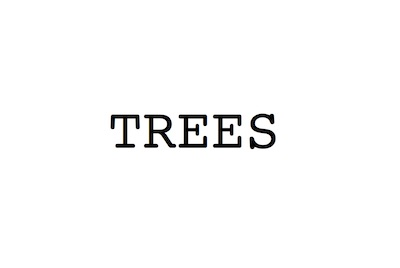
\includegraphics[width=0.5\textwidth]{img.jpg}

\begin{problems}

\problem  % Problem 1

\begin{problemparts}
\problempart % Problem 1a
DAG Relaxation order: $[(a,b),(a,d),(d,b),(d,e),(b,c),(b,e),(b,f),(e,f),(f,c)]$

Dijkstra order: $[(a,b),(a,d),(b,c),(b,e),(b,f),(f,c),(e,f),(d,b),(d,e)]$

\problempart % Problem 1b
Both algorithms output the same shortest-path results:

$\delta(a,a)=0$ 

$\delta(a,b)=2$ 

$\delta(a,c)=3$ 

$\delta(a,d)=6$ 

$\delta(a,e)=5$ 

$\delta(a,f)=4$

\end{problemparts}

\newpage
\problem  % Problem 2
We assume that the graph could contain negative cycles and negative weights, since this is not mentioned in the problem statement. We are given that the shortest path to each vertex traverses at most $k$ edges, but we do not know what $k$ is. Since we can obtain the shortest paths using at most $k'$ edges (the $k'$-th layer of the constructed graph $G'$ for Bellman-Ford), we can modify Bellman-Ford to only construct the duplicated graph layers incrementally then relaxing edges into the new layer, rather than constructing the entire graph $G'$ initially. Since we do not know the value of $k$, the criteria for termination will be when the $k'$-edge shortest path distance do not change between layers.

We prove by induction on layer $i$ of $G'$ that this algorithm correctly computes $\delta(s_0, v_{i+1})$ for all $v \in V$. We first initialize $G'$ as containing only the first layer ($v_0: \forall v \in V)$ and $\delta$ initialized to 0 for $(s_0,s_0)$, and $\infty$ otherwise. This proves the base case, since in layer $i=0$, only the source is reachable ($\delta(s_0,s_0)=0$), and every other vertex is not reachable ($\delta(s_0, v_0)=\infty$, for all $v \in V$).

In the inductive step, we assume that $G'$ contains layers from $0 \ldots i$ and $\delta(s_0,v_j)$ have been computed for all $v \in V$ and $j \in \{0,\ldots,i\}$. We append layer $i+1$ by adding vertices $v_{i+1}$ for $v \in V$ and their associated edges from layer $i$. This new layer does not affect distances in previous layers since they come later in the topological sort order. So applying DAG Relaxation on the new edges out of the vertices in layer $i$ correctly computes $\delta(s_0,v_{i+1})$ for all $v \in V$.

Since we know that the shortest path from $s$ to any vertex uses at most $k$ edges, we will eventually reach the layer $i$ with at most $k'$ edges such that $k' \geq k$ and $\delta(s_0,v_{k'})=\delta(s_0,v_{k'+1})$ for all $v \in V$. When this condition first occurs, we terminate the algorithm and output $\delta(s,v)=\delta(s_0,v_k)$ for all $v \in V$.

We need to construct $k+1$ layers of $G$, and each layer takes $O(|E|)$ time for DAG relaxation, therefore, this algorithm runs in $O(|V|+k|E|)$ time in the worst case, as required. Since the graph is connected, $|V|=O(|E|)$, and the running time can be abbreviated to $O(k|E|)$.

\newpage
\problem  % Problem 3
We first construct a graph $G_1$, where the clearings of the problem are represented as vertices, and slopes as edges. We only include those clearings and slopes which have a decreasing elevation from one to another. We also construct a graph $G_2$, which is constructed similarly to $G_1$, except that it uses the elevation of clearings after the dynamite located in that clearing has been detonated.

We add a directed edge between $D_1$ and $D_2$ the vertices of $G_1$ and $G_2$ respectively, where the detonator is located. This edge represents Bames choosing to detonate, and has a weight of 0. We also add a supernode $S$, which has two incoming edges of weight 0 from $S_1$ and $S_2$, which represent Bames reaching the target either through not detonating ($S_1$) or detonating ($S_2$). Let us call this combined graph $G$.

Since the elevations are strictly decreasing until clearing $S_1,S_2$, then $G$ must be a DAG. We can use DAG Relaxation from source $L_1$ to $S$, with the shortest path being equivalent by definition to the minimum distance for Bames to reach $S$, with or without detonation, and always on a decreasing elevation path. Graph $G$ has $2n+1=O(n)$ vertices and edges, so DAG Relaxation on $G$ runs in $O(n)$.

\newpage
\problem  % Problem 4
It is easier to determine the existence of non-zero weight cycles, rather than showing that zero weight cycles exist in a graph. Therefore, we construct a graph $G$ with particle locations as vertices and transitions as edges. Add a supernode $s$ with 0 weight to each vertex to ensure that the entire $G$ is a single connected component. 

Now we can run Bellman-Ford to detect negative weight cycles in $G$. Next, negate all edge weights (transition weights) in $G$ and run Bellman-Ford a second time to determine if there are any positive weight cycles in the negated edge weight graph of $G$. If either of these two runs of Bellman-Ford produce a non-zero weight cycle, then the force field is not conservative. Otherwise, no non-zero weight cycles exist, and we can return that the force field is conservative.

Since there are $n+1=O(n)$ vertices in $G$ and $O(n)$ edges, two runs of Bellman-Ford give a worst-case running time of $O(n^2)$ as desired.

\newpage
\problem  % Problem 5
Create a graph $G$, with the vertices representing an intersection. Each intersection is represented by $g$ vertices $v_i$, with $i \in \{1,\ldots,g\}$. Vertex $v_i$ represents being at that intersection with $i$ units of gas in her tank.

Edges in $G$ represent roads. For any bidirectional road connecting intersections $u,v$, let $t(u,v)$ be the driving time of the road, and $e(u),e(v)$ be the elevation of intersections $u,v$ respectively. Without loss of generality, assume $e(u) < e(v)$ for the three cases when constructing edges in graph $G$:
\begin{itemize}
    \item Down-hill road edges: add a weight $t(u,v)$ edge $(v_i,u_i)$ for every $i \in \{1,\ldots,g\}$ since travelling in this direction requires no gas.
    \item Up-hill road edges: if $e(u)=e(v)$, add an edge in the same way as for down-hill edges. Otherwise, add a weight $t(u,v)$ edge $(u_i,v_{i-l})$ for every $i \in \{l+1,\ldots,g\}$ since going up-hill requires gas and she cannot have a negative tank.
    \item Gas station edges: for each gas station at intersection $v$, add a weight $t_G$ edge $(v_i, v_{i+1}$ for every $i \in \{1,\ldots,g-1\}$ corresponding to filling up the tank by one unit at the gas station.
\end{itemize}

This graph has the property that any path from vertex $s_g$ to any vertex $t_i$ for $i \in \{1,\ldots,g\}$ will be a valid route from source to destination, never having a nonempty tank along the way. The weighted shortest path corresponds to the minimum time required to reach the destination. So we can use a SSSP algorithm from $s_g$ to $t_i$ for all $i \in \{1,\ldots,g\}$, and return a path with minimum weight (or return no such path exists). This graph may have cycles, but only positive edge weights, so Dijkstra can be used.

Since the average degree of each intersection is bounded by a constant and every road connects two intersections, then $2r<5n$ and $r=O(n)$. Since $g<n$ by the problem statement, $G$ has $O(n^2)$ vertices and $O(n^2)$ edges, so it takes $O(n^2)$ time to construct. Then Dijkstra takes $O(n^2\log (n^2)+n^2)=O(n^2\log n)$ time in total, as required.

\newpage
\problem  % Problem 6
Programming question only.

\end{problems}

\end{document}
